\documentclass[12pt]{article}
\usepackage{url,graphicx,tabularx,array,geometry, extramarks, fancyhdr, lastpage,amsthm, amsmath, amssymb, mathtools}
\setlength{\parskip}{1ex} %--skip lines between paragraphs
%\setlength{\parindent}{10pt} %--don't indent paragraphs
\setlength\parindent{24pt}

%-- Commands for header
\renewcommand{\title}[1]{\textbf{#1}\\}
\renewcommand{\line}{\begin{tabularx}{\textwidth}{X>{\raggedleft}X}\hline\\\end{tabularx}\\[-0.5cm]}
\newcommand{\leftright}[2]{\begin{tabularx}{\textwidth}{X>{\raggedleft}X}#1%
& #2\\\end{tabularx}\\[-0.5cm]}

% Set up the header and footer
\pagestyle{fancy}
\lhead{\hmwkAuthorName} % Top left header
%\chead{\hmwkClass\  \hmwkTitle} % Top center head
\rhead{\hmwkDueDate} % Top right header
\lfoot{\lastxmark} % Bottom left footer
\cfoot{} % Bottom center footer
\rfoot{Page\ \thepage\ of\ \protect\pageref{LastPage}} % Bottom right footer
\renewcommand\headrulewidth{0.4pt} % Size of the header rule
\renewcommand\footrulewidth{0.4pt} % Size of the footer rule

\newcommand{\hmwkTitle}{HW\ \#4} % Assignment title
\newcommand{\hmwkDueDate}{\ May\ 14,\ 2014} % Due date
\newcommand{\hmwkClass}{STAT\ 243} % Course/class
%\newcommand{\hmwkClassTime}{10:30am} % Class/lecture time%
%\newcommand{\hmwkClassInstructor}{Jones} % Teacher/lecturer%
\newcommand{\hmwkAuthorName}{Angela Andrews, Nicholas Lytal} % Your name%leftright{\today}{Angela Andrews} %-- left and right positions in the header

\newcommand{\partdiv}[2]{\frac{\partial #1}{\partial #2}}
\newcommand{\logpart}[1]{\frac{\partial l_R}{\partial #1}}
\newcommand{\logpartsq}[1]{\frac{\partial^2 l_R}{\partial #1}}
\newcommand{\Pmat}{A(A'VA)^{-1}A'}
\newcommand{\partp}{\frac{\partial P}{\partial \theta_i}}
\newcommand{\ppartial}{-P\partdiv{V}{\theta_i}P}
\newcommand{\lo}{\mathrm{log}}
\newcommand{\tone}{\theta_1}
\newcommand{\ttwo}{\theta_2}
%\linespread{2} %-- Uncomment for Double Space
\begin{document}

\center{\title{STAT 243 HW\#4}}

\begin{description}

%%%%%%%%
% Problem 1  %
%%%%%%%%

\item[1.] We use the Monte Carlo method to evaluate each of the following integrals:
\begin{description}
\item[a.] \[\int_0^1 x^2 dx\]

Here, we let $f(x) = \frac{1}{1-0}$, a Uniform(0,1) distribution, and we let $h(x) = x^2$. We take 1,000,000 samples from a Uniform(0,1), and using the Monte Carlo method we obtain an estimate of the evaluated integral as .333328, or equivalenty $\frac{1}{3}$.

\item[b.] \[\int_0^1 \int^2_{-2} x^2 \mathrm{cos}(xy) \ \ dx dy\]

Here, since we have two variables, instead of having $f(x)$ and $h(x)$, we will instead have $f(x,y)$ and $h(x,y)$. Here, we let $f(x,y) = \frac{1}{4}$ and we let $h(x,y) = 4x^2\mathrm{cos}(xy)$. Thus, we see that $\int_0^1 \int_{-1}^2 \frac{1}{4} = 1$, which satisfies our condition for $f(x,y)$. We sample from a Uniform(-2,2) for x and from a Uniform(0,1) for y, each 1,000,000 times, and we plug these values into our function $h(x,y)$. Thus, taking 1,000,000 samples from the two Uniform distribution and using the Monte Carlo method, we obtain an estimate of the evaluated integral of 3.480481.

\item[c.] \[\int_0^\infty \frac{3}{4} e^{-\frac{x^3}{4}} dx\]

Here, we see that the integral is over a very large range (0 to $\infty$), compared to the other integrals that we have evaluated. As a result, we do not expect to obtain as accurate results for evaluating the integral as we did in parts a and b. Thus, here we estimate the integral 100 times using 1,000,000 samples and the Monte Carlo method, and plot the density to see the value that the estimates center themselves around. For this integral, we let $f(x)$ and $h(x)$ be defined as:

\[f(x) = \frac{\frac{1}{4}^5}{\Gamma(5)} \cdot x^4 \mathrm{exp}\left(-\frac{x}{4} \right) \sim \mathrm{Gamma}(5, 0.25)\]

\[h(x) = \frac{3}{4} \cdot \frac{\Gamma(5)}{\frac{1}{4}^5} \cdot \mathrm{exp} \left( \frac{x}{4} - \frac{x^3}{4}\right)\]

Thus, we take 1,000,000 samples of x from $x \sim \Gamma(5, 0.25)$ and plug these into $h(x)$ to be used in the formula for estimating the integral. Repeating this process 1000 times, we obtain the following density plot of evaluated integral estimates. The vertical red line represents the maximum of the density, which occurs at the value 2.25775.

\[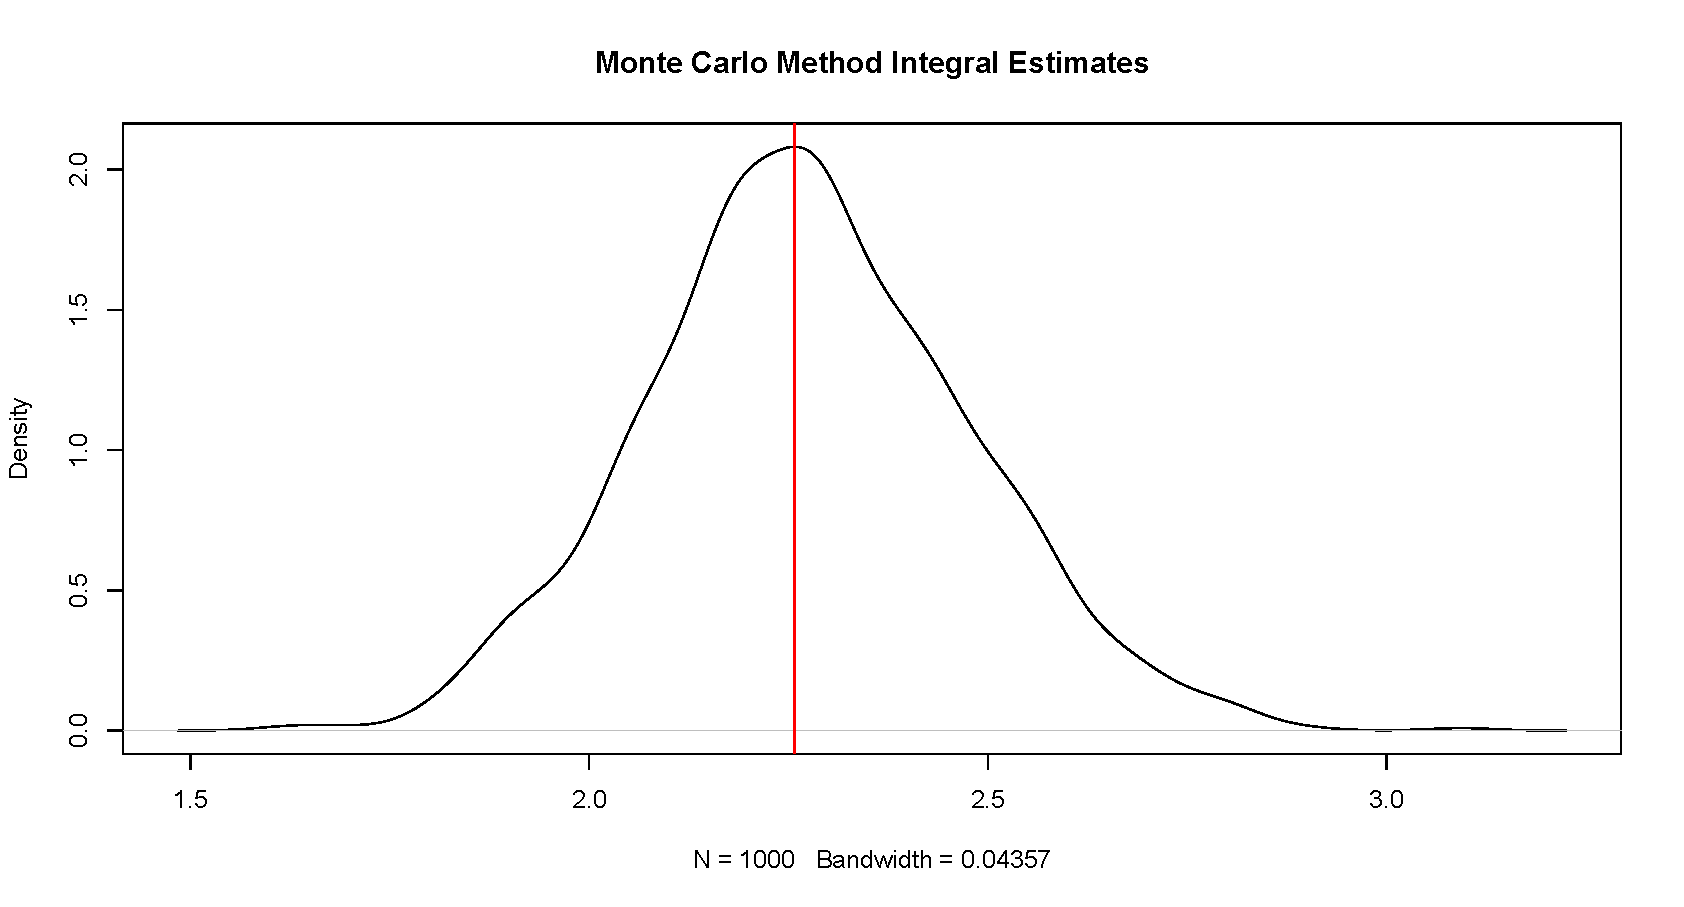
\includegraphics[scale = 0.50]{STA243HW4Plot1}\]
\end{description}

%%%%%%%%
% Problem 2  %
%%%%%%%%
\item[2.] We let
\[I = \frac{1}{\sqrt{2\pi}} \int_1^2 e^{-\frac{x^3}{2}}dx\]
and estimate $I$ using importance sampling. We take $g$ to be $N(1.5, \nu^2)$ with $\nu = 0.1$ and 10. 


%%%%%%%%
% Problem 3  %
%%%%%%%%

\item[3.] We will approximate the following integral using both the simple Monte Carlo integration and the control variate method:
\[I = \int_0^1 \frac{1}{1 + x} dx\]

\begin{description}
\item[a.]We let $h(x) = \frac{1}{1+x}$ and $U_1, \dots U_n$ be iid Unif[0,1]. 
\item[b.]
\item[c.]
\item[d.]
\end{description}


%%%%%%%%
% Problem 4  %
%%%%%%%%

\item[4.] We consider a common application in statistics: three different treatments are to be compared by applying them to a randomly selected experimental units. However; instead of the usualy assumption associated with $e_{ij}$ in the typical analysis of variance methods of comparison, we assume that the $e_{ij}$  have independent and identical double exponential distributions centered on zero.
\begin{itemize}
\item[a.]
\item[b.]
\end{itemize}


%%%%%%%%
% Problem 5  %
%%%%%%%%

\item[5.] We consider the zero-inflated Poisson( ZIP) model, in which random data $X_1, \dots, X_n$ are assumed to be of the form $X_i = R_iY_i$, where $Y_i$'s have a Poisson($\lambda$) distribution and the $R_i$'s have a Bernoulli($p$) distribution, all independent of each other. Given an outcome $x = (x_1, \dots, x_n)$, the objective is to estimate both $\lambda$ and $p$. We consider the following hierarchical Bayes model:
\begin{itemize}
\item $p \sim$ Uniform(0,1) (prior for $p$)
\item $(\lambda | p) \sim$ Gamma$(a, b)$ (prior for $\lambda$)
\item $(r_i | p, \lambda) \sim$ Bernoulli($p$) independently (from the model above)
\item $(x_i | r, \lambda, p) \sim$ Poisson($\lambda r_i$) independently (from the model above)
\end{itemize}
where $a$ and $b$ are known parameters, and $r = (r_1, \dots, r_n)$. It follows that:
\[f(x, r, \lambda, p) = \frac{b^a\lambda^{a-1}e^{-b\lambda}}{\Gamma(a)}\prod^n_{i = 1} \frac{e^{-\lambda r_i} (\lambda r_i)^{x_i}}{x_i!} p^{r_i} (1 - p)^{1 - r_i}\]

We wish to sample from the posterior pdf $f(\lambda, p, r | x)$ using the Gibbs sampler.\
\begin{description}
\item[a.]
\item[b.]
\item[c.]
\end{description}

%%%%%%%%
% Problem 6  %
%%%%%%%%

\item[6. ] The Independence - Metropolis - Hastings Algorithm is an importance-sampling version of MCMC. We draw the proposal from a fixed distribution $g$. Generally, $g$ is chosen to be an approximation to $f$. The acceptance probability becomes:
\[r(x, y) = min\left\{ \frac{f(y)}{f(x)} \cdot \frac{g(x)}{g(y)}, 1 \right\}\]

A random variable Z has an inverge Gaussian distribution it it has density

\[f(z) \propto z^{-3/2} \mathrm{exp}\left\{ -\theta_1z - \frac{\theta_2}{z} + 2\sqrt{\theta_1\theta_2} + \lo \sqrt{2\theta_2}\right\}, \ \ z >0\]

where $\theta_1 0$ and $\theta_2 >0$ are parameters. It can be shown that 
\[E(Z) = \sqrt{\frac{\theta_2}{\theta_1}} \ \ \ \ \mathrm{and} \ \ \ \ E\left(\frac{1}{Z} \right)= \sqrt{\frac{\theta_1}{\theta_2}} + \frac{1}{2\theta_2}\]

We let $\theta_1 = 1.5$ and $\theta_2 = 2$, and draw a sample of size 1,000 using the independence-Metropolis-Hastings algroithm. We use a Gamma distribution as the proposal density. 
\end{description}
\end{document}


